%versi 3 (22-07-2020)
\chapter{Landasan Teori}
\label{chap:teori}
Pada bab ini akan menjelaskan dasar teori mengenai Portal Akademik Mahasiswa dan Selenium. 

\section{Portal Akademik Mahasiswa 2018}
\label{sec:pam} 
Portal Akademik Mahasiswa (selanjutnya disingkat dengan PAM) adalah sebuah \textit{web} yang di peruntukan bagi mahasiswa dalam rangka mendapatkan informasi kegiatan akademik mulai dari registrasi, melihat jadwal kuliah dan ujian, info nilai sampai pendaftaran sidang\cite{portalunpar}. Portal Akademik Mahasiswa dapat diakses melalui \url{https://studentportal.unpar.ac.id/}. 

\begin{figure}[H]
	\centering
	
\includegraphics[scale=0.4]{Gambar/halaman2018.jpg}
	\caption{Tampilan halaman awal Portal Akademik Mahasiswa} 
	\label{fig:studpor_home_2018}
\end{figure}

Pada Gambar \ref{fig:studpor_home_2018} adalah tampilan awal ketika masuk ke halaman \url{https://studentportal.unpar.ac.id/}. Mahasiswa perlu melakukan \textit{login} dengan \textit{email} dan \textit{password} mahasiswa UNPAR untuk dapat menggunakan fitur-fitur yang tersedia seperti:
\begin{enumerate}
	\item Fitur mengisi form rencana semester (FRS) atau melakukan perubahan rencana studi (PRS) secara online \\
	Panduan untuk melakukan FRS/PRS online.
	\begin{enumerate}
		\item Masuk ke halaman \url{https://studentportal.unpar.ac.id/} lalu klik tombol ``\textit{Login}'' yang dapat dilihat pada Gambar \ref{fig:studpor_home_2018}
		\item Lakukan ``\textit{Login}'' dengan memasukan email dan password mahasiswa UNPAR pada halaman sso.
		\begin{figure}[H]
			\centering
			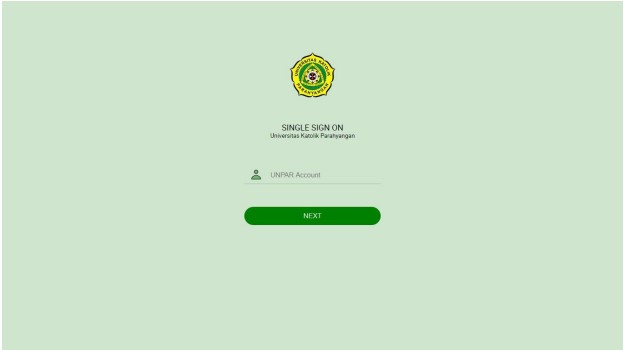
\includegraphics[scale=0.7]{Gambar/sso2018.jpg}
			\caption{Tampilan halaman untuk memasukan \textit{email} Portal Akademik Mahasiswa} 
			\label{fig:sso_2018}
		\end{figure}
	
		\begin{figure}[H]
			\centering
			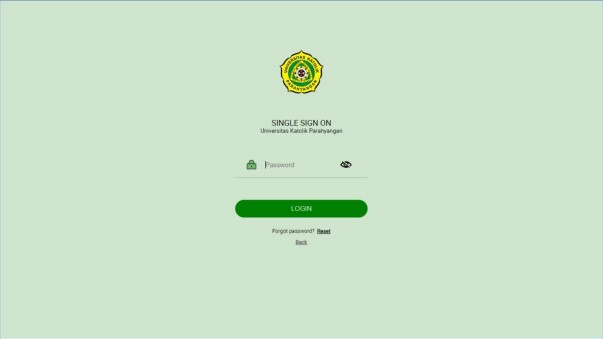
\includegraphics[scale=0.7]{Gambar/pass2018.jpg}
			\caption{Tampilan halaman untuk memasukan \textit{password} Portal Akademik Mahasiswa} 
			\label{fig:pass_2018}
		\end{figure}
		\item Ketika \textit{login} telah berhasil, maka browser akan menampilkan halaman utama, lalu klik pada heksagon berlabel `FRS/PRS' untuk melakukan FRS/PRS online.
		\begin{figure}[H]
			\centering
			
\includegraphics[scale=0.7]{Gambar/frs2018.jpg}
			\caption{Tampilan halaman setelah berhasil \textit{login}} 
			\label{fig:frs_2018}
		\end{figure}
		\item Mahasiswa dapat melakukan FRS sesuai waktu yang sudah ditentukan atau mahasiswa dapat melakukan PRS setelah FRS selesai dan sesuai waktu yang sudah ditentukan untuk PRS.		
	\end{enumerate}
	
	\item Fitur Profil Mahasiswa
	Panduan untuk melihat profil mahasiswa.
	 \begin{enumerate}
	 	\item Mahasiswa melakukan \textit{login} terlebih dahulu. 
	 	\item Menekan menu ``PROFIL'' pada halaman setelah berhasil login seperti pada Gambar \ref{fig:frs_2018}. 
	 	\item Mahasiswa dapat melihat informasi data diri di halaman profil mahasiswa.
	 	\begin{figure}[H]
	 		\centering
	 		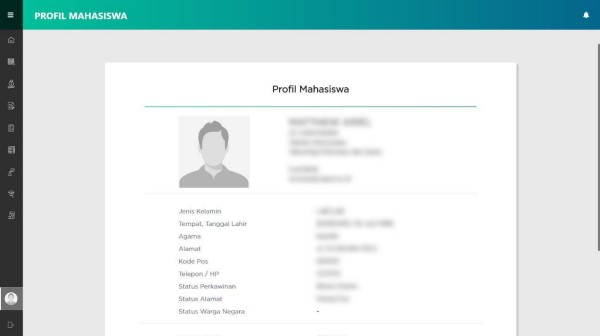
\includegraphics[scale=0.7]{Gambar/profil2018.jpg}
	 		\caption{Tampilan halaman profil mahasiswa} 
	 		\label{fig:profil_2018}
	 	\end{figure}
 	\end{enumerate}
 
	\item Fitur Pembayaran
	Panduan untuk melihat informasi pembayaran.
	\begin{enumerate}
		\item Mahasiswa melakukan \textit{login} terlebih dahulu. 
		\item Menekan menu ``PEMBAYARAN'' pada halaman setelah berhasil login seperti pada Gambar \ref{fig:frs_2018}. 
		\item Pada halaman pembayaran, mahasiswa dapat melihat informasi pembayaran yang terdiri dari Tagihan Pembayaran, Riwayat Pembayaran, dan Keterangan.
	\end{enumerate}
	Pada Gambar \ref{fig:bayar_2018} adalah tabel ``Tagihan Pembayaran'' yang menampilkan jenis tagihan dan jumlah tagihan dari setiap jenis tagihan yang ada.
	\begin{figure}[H]
		\centering
		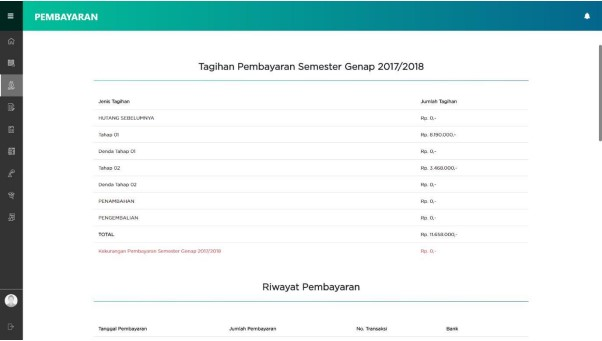
\includegraphics[scale=0.7]{Gambar/bayar2018.jpg}
		\caption{Tampilan halaman pembayaran bagian Tagihan Pembayaran} 
		\label{fig:bayar_2018}
	\end{figure}\\
	
	Pada Gambar \ref{fig:riw_2018} adalah tabel ``Riwayat Pembayaran'' yang menampilkan histori pembayaran yang telah dilakukan.
	\begin{figure}[H]
		\centering
		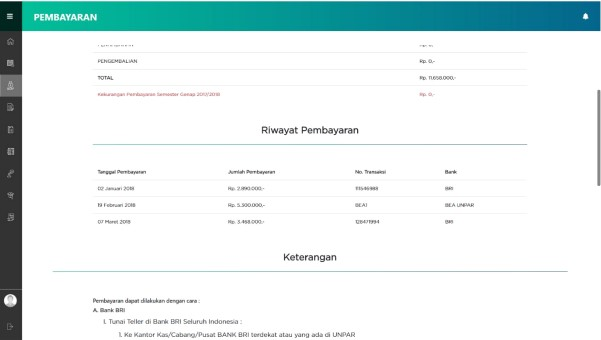
\includegraphics[scale=0.7]{Gambar/riwayat2018.jpg}
		\caption{Tampilan halaman pembayaran bagian Riwayat Pembayaran} 
		\label{fig:riw_2018}
	\end{figure}\\
	
	Pada Gambar \ref{fig:ketbayar_2018} adalah tabel ``Keterangan'' yang menampilkan tata cara pembayaran yang dapat dilakukan untuk melakukan pembayaran.
	\begin{figure}[H]
		\centering
		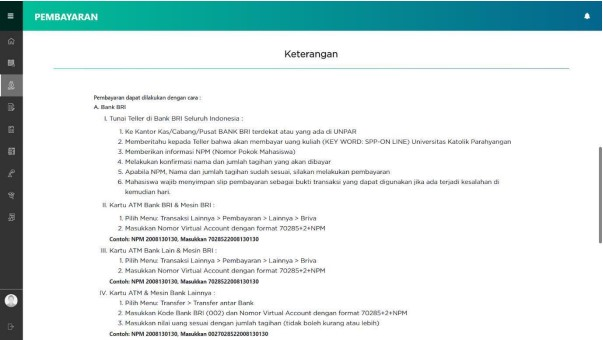
\includegraphics[scale=0.7]{Gambar/keterangan2018.jpg}
		\caption{Tampilan halaman pembayaran bagian Keterangan} 
		\label{fig:ketbayar_2018}
	\end{figure}
	\item Fitur Nilai
	Panduan untuk melihat informasi nilai mahasiswa.
	\begin{enumerate}
		\item Mahasiswa melakukan \textit{login} terlebih dahulu. 
		\item Menekan menu ``NILAI'' pada halaman setelah berhasil login seperti pada Gambar \ref{fig:frs_2018}. 
		\item Pada halaman nilai, mahasiswa dapat melihat informasi nilai dari setiap mata kuliah yang diambil.
		\begin{figure}[H]
			\centering
			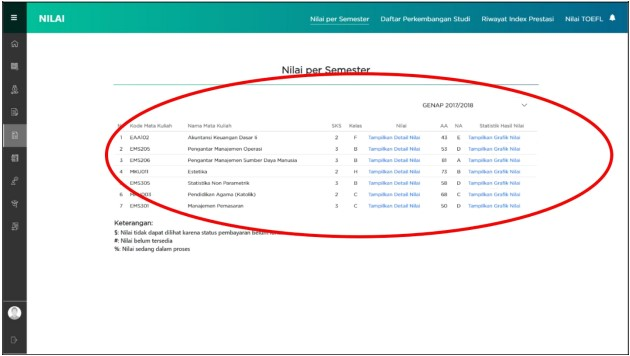
\includegraphics[scale=0.7]{Gambar/nilai2018.jpg}
			\caption{Tampilan halaman nilai bagian Nilai per Semester} 
			\label{fig:nilai_2018}
		\end{figure}
		\item Mahasiswa dapat mengakses menu ``Riwayat Index Prestasi'' untuk melihat `IPK' dan `IPS' mahasiswa.
		\begin{figure}[H]
			\centering
			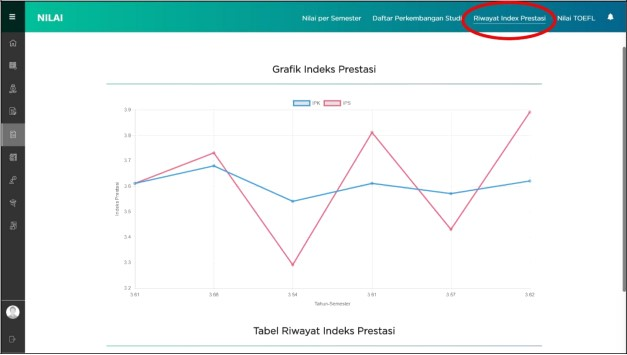
\includegraphics[scale=0.7]{Gambar/rip2018.jpg}
			\caption{Tampilan halaman nilai bagian Riwayat Index Prestasi} 
			\label{fig:rip_2018}
		\end{figure}
	\end{enumerate}	
\end{enumerate}

\section{Selenium}
\label{sec:selenium}
Selenium adalah \textit{open-source} \textit{framework} pengujian otomatisasi untuk aplikasi web\cite{selenium}. Selenium ini adalah WebDriver yang merupakan sebuah \textit{interface} untuk menulis suatu instruksi yang dapat dijalankan secara otomatis dan bergantian pada \textit{browser}. Otomatisasi pengujian situs web dapat menggunakan API WebDriver. WebDriver menggunakan API otomatisasi \textit{browser} yang disediakan oleh vendor \textit{browser} untuk mengontrol \textit{browser} dan melakukan pengujian. API WebDriver ini seolah-olah membuat pengguna secara langsung mengoperasi \textit{browser}, padahal dijalankan secara otomatis langsung oleh \textit{API} WebDriver tersebut. Selenium WebDriver adalah sebuah \textit{tools} yang berguna untuk melakukan otomatisasi terhadap web pada \textit{browser}. Selenium WebDriver ini tersedia untuk bahasa pemrograman Ruby, Java, Python, C\#, dan JavaScript. 

\subsection{Navigasi}
Hal pertama untuk menggunakan WebDriver adalah melakukan navigasi ke situs web. Cara normal untuk melakukan navigasi adalah dengan \textit{method} \textit{get}().
\begin{lstlisting}[language=python, caption=Contoh kode untuk membuka situs web, label=kode:2:navigate]
	driver.get("https://selenium.dev")
\end{lstlisting}

\subsection{Menemukan elemen}
Salah satu teknik mendasar untuk dipelajari saat menggunakan WebDriver adalah cara menemukan elemen di halaman web. WebDriver menawarkan sejumlah tipe pemilih bawaan, di antaranya menemukan elemen dengan atribut ID.
\begin{lstlisting}[language=python, caption=Contoh kode untuk menemukan elemen dengan atribut ID, label=kode:2:elemenid]
	driver.find_element(By.ID, "cheese")	
	driver.find_element_by_id("cheese")
\end{lstlisting}
Kode \ref{kode:2:elemenid} merupakan 2 contoh kode yang dapat digunakan untuk menemukan elemen berdasarkan atribut ID. Terdapat delapan strategi lokasi elemen bawaan yang berbeda di WebDriver:
\begin{enumerate}
	\item class name: Menemukan elemen yang nama kelasnya berisi nilai pencarian (nama kelas gabungan tidak diizinkan).
	\item css selector: Menemukan elemen yang cocok dengan pemilih CSS.
	\item id : Menemukan elemen yang atribut ID-nya cocok dengan nilai pencarian.
	\item name: Menemukan elemen yang atribut NAME-nya cocok dengan nilai pencarian. 
	\item link text: Menemukan elemen jangkar yang teksnya terlihat cocok dengan nilai pencarian. 
	\item partial link text: Menemukan elemen jangkar yang teksnya terlihat berisi nilai pencarian. Jika beberapa elemen cocok, hanya yang pertama yang akan dipilih.
	\item tag name: Menemukan elemen yang nama tagnya cocok dengan nilai pencarian.
	\item xpath: Menemukan elemen yang cocok dengan ekspresi XPath.
\end{enumerate}
Selenium 4 menghadirkan \textit{Relative Locator} yang sebelumnya disebut \textit{Friendly Locators}. Fungsi ini ditambahkan untuk membantu menemukan elemen yang berdekatan dengan elemen lain. Pencari Relatif yang Tersedia adalah:
\begin{enumerate}
	\item above: Mengembalikan WebElement, yang muncul di atas elemen yang ditentukan.
	\begin{lstlisting}[language=python, caption=Contoh kode Pencari Relatif Above, label=kode:2:above]
		from selenium.webdriver.common.by import By
		from selenium.webdriver.support.relative_locator import locate_with
		
		passwordField = driver.find_element(By.ID, "password")
		emailAddressField = driver.find_element(locate_with(By.TAG_NAME, "input").above(passwordField))
	\end{lstlisting}
	\item below: Mengembalikan WebElement, yang muncul di bawah elemen yang ditentukan.
	\begin{lstlisting}[language=python, caption=Contoh kode Pencari Relatif Below, label=kode:2:below]
		from selenium.webdriver.common.by import By
		from selenium.webdriver.support.relative_locator import locate_with
		
		emailAddressField = driver.find_element(By.ID, "email")
		passwordField = driver.find_element(locate_with(By.TAG_NAME, "input").below(emailAddressField))
	\end{lstlisting}
	\item toLeftOf: Mengembalikan WebElement, yang muncul di sebelah kiri elemen yang ditentu.
	\begin{lstlisting}[language=python, caption=Contoh kode Pencari Relatif toLeftOf, label=kode:2:left]
		from selenium.webdriver.common.by import By
		from selenium.webdriver.support.relative_locator import locate_with
		
		submitButton = driver.find_element(By.ID, "submit")
		cancelButton = driver.find_element(locate_with(By.TAG_NAME, "button").
		to_left_of(submitButton))
	\end{lstlisting}
	\item toRightOf: Mengembalikan WebElement, yang muncul di sebelah kanan elemen yang ditentukan.
	\begin{lstlisting}[language=python, caption=Contoh kode Pencari Relatif toRightOf, label=kode:2:right]
		from selenium.webdriver.common.by import By
		from selenium.webdriver.support.relative_locator import locate_with
		
		cancelButton = driver.find_element(By.ID, "cancel")
		submitButton = driver.find_element(locate_with(By.TAG_NAME, "button").
		to_right_of(cancelButton))
	\end{lstlisting}
	\item near: Mengembalikan WebElement, yang paling jauh 50px dari elemen yang ditentukan.
	\begin{lstlisting}[language=python, caption=Contoh kode Pencari Relatif Near, label=kode:2:near]
		from selenium.webdriver.common.by import By
		from selenium.webdriver.support.relative_locator import locate_with
		
		emailAddressLabel = driver.find_element(By.ID, "lbl-email")
		emailAddressField = driver.find_element(locate_with(By.TAG_NAME, "input").
		near(emailAddressLabel))
	\end{lstlisting}
\end{enumerate}	

\subsection{Waits}
WebDriver secara umum dapat dikatakan memiliki API pemblokiran. Karena ini adalah \textit{library} di luar proses yang menginstruksikan browser apa yang harus dilakukan, dan karena platform web secara intrinsik memiliki sifat asinkron, WebDriver tidak melacak status document object model (DOM) yang aktif dan real-time. Selenium WebDriver memiliki tiga tipe waits:
\begin{enumerate}
	\item Implicit wait: memberi tahu WebDriver untuk melakukan polling DOM selama jangka waktu tertentu ketika mencoba menemukan elemen atau elemen jika tidak segera tersedia. Pengaturan default adalah 0, artinya dinonaktifkan. Setelah disetel, penantian implisit disetel untuk masa pakai sesi.
	\begin{lstlisting}[language=python, caption=Contoh kode Implicit wait, label=kode:2:implicit]
		driver = Firefox()
		driver.implicitly_wait(10)
		driver.get("http://somedomain/url_that_delays_loading")
		my_dynamic_element = driver.find_element(By.ID, "myDynamicElement")
	\end{lstlisting}
	\item Explicit wait: mengizinkan kode untuk menghentikan eksekusi program, atau membekukan \textit{thread}, hingga suatu kondisi dapat teratasi. Kondisi ini dipanggil dengan frekuensi tertentu sampai batas waktu tunggu terlewati.
	\begin{lstlisting}[language=python, caption=Contoh kode Explicit wait, label=kode:2:explicit]
		from selenium.webdriver.support.ui import WebDriverWait
		
		driver.navigate("file:///race_condition.html")
		el = WebDriverWait(driver).until(lambda d: d.find_element_by_tag_name("p"))
		assert el.text == "Hello from JavaScript!"
	\end{lstlisting}
	\item Fluent wait: menentukan jumlah waktu maksimum untuk menunggu suatu kondisi, serta frekuensi untuk memeriksa kondisi tersebut.
	\begin{lstlisting}[language=python, caption=Contoh kode FluentWait, label=kode:2:FluentWait]
		driver = Firefox()
		driver.get("http://somedomain/url_that_delays_loading")
		wait = WebDriverWait(driver, 10, poll_frequency=1, ignored_exceptions=[ElementNotVisibleException, ElementNotSelectableException])
		element = wait.until(EC.element_to_be_clickable((By.XPATH, "//div")))
	\end{lstlisting}
\end{enumerate}










